\chapter{Lab 2}
\setcounter{TASignatures}{0}
\setcounter{AsideCounter}{0}

\section{Introduction}
    \vspace{0.1em}

    \textbf{In this lab you gain experience with:}
    \begin{enumerate}
        \item Analyzing how a multi-rung ladder logic program will execute
        \item Using the output Latch (OTL)
        \item Using the output Unlatch (OTU)
        \item Storing the result of a rung in a tag
        \item Accomplishing logical functionality using on a multi-scan approach
    \end{enumerate}

\subsection{Lab Files}

Go to iLearn and download the PLC and HMI files for this lab to the PC. Then download the PLC project to the PLC and the HMI application to the HMI. 

\subsection{Acceptable Instructions}

You may have previous experience with PLCs and that is great! However, you are only allowed to use the instructions that we have covered thus far in the lab. So, if you have experience already, consider it a challenge to restrict yourself to only use the instructions that have been covered thus far in lecture to solve the problem!

\subsection{How to Interface with the PLC and HMI}
\begin{samepage}
\noindent If you are unclear on any of the following, refer to the Lab 1 Manual:
\begin{enumerate}
    \item Download to the PLC
    \item Go online with the PLC
    \item Put the PLC into Run Mode
    \item Make online and offline edits to the PLC program
    \item Download to the HMI
    \item Toggle a boolean tag
\end{enumerate}

\end{samepage}

\subsection{How to get credit}
The \textbf{pre-lab must be submitted to the TA before beginning work on the lab}. If it is not complete then you will be required to complete the pre-lab before you are allowed to begin working on the lab.

In order to get credit for completing each part of this lab, \textbf{you must personally read and complete each portion of the lab and demonstrate the completion to the TA}. Each section has one or more signature slots that must be signed by the TA to confirm that the section was completed. Each section is worth equal credit. 

\subsection{20 minute grace period}
To receive full credit, the lab must be completed and demonstrated during the assigned lab time. However, if you cannot complete the lab within that time, you can complete and demonstrate the lab within the first 20 minutes of the subsequent lab time and still receive full credit. \textbf{If the lab is not completed within the assigned lab time and is not completed within the 20 minute grace period, then the lab is considered late}. If you submit the lab late, then there will be a 20\% deduction compounded weekly.


\subsection{Lab agreement}

The planning of a program is often a very social activity, however the actual writing of the code is always an individual pursuit. In this class it is very much the same. Students are welcome to verbally assist each other, but each person is required to write their own code and personally complete each lab. In this way each student will gain valuable experience with programming PLCs. 

\textbf{The undersigned person guarantees that any and all work demonstrated to the TA in regard to this lab is a result of their own work with no unauthorized help.}

\signatureSlot{Student (Print \& Sign)}



\section{Box Transfer System}

This section corresponds to the \verb|Lab2_1| object in the Lab2 PLC file. \textbf{You will have to create tags to be able to build a bit latch sequence as demonstrated in lecture}.
\\ 
\\

Congratulations are in order. You have just landed a big contract with a certain online retailer that ships thousands of packages a day (you know the one). They have a heavy parcel moving machine that they use to transfer heavy packages from their conveyor to the truck. However, at the moment the machine must be controlled by a human operator. The online retailer has tasked you with automating the task. 


\subsection{How should the logic work?}


They want you to write a ladder logic program that will be initiated by a button connected to a signal in the PLC called \verb|Start_Transfer|. When \verb|Start_Transfer| is pressed, the parcel mover will go vertically up until it reaches a switch called \verb|Transfer_Raised|. Then it will move horizontally until it reaches the switch called \verb|Transfer_Extended|. Then the transfer will lower until it reaches the \verb|Transfer_Lowered| switch. 

\aside{Machines like this heavy parcel transfer system are typically pneumatically driven. Each of the motions made possible by a pneumatic cylinder. Each of the cylinders is connected to pneumatic valves which are controlled by the PLC. Pneumatic cylinder control is the most common way to implement motion in factories today!}

In order to tell the heavy parcel transfer machine to raise, extend, and lower use the \verb|Raise_Transfer|, \verb|Extend_Transfer|, and \verb|Lower_Transfer| signals respectively. The transfer movement doesn't happen immediately. Rather, you must hold the command for a full second before the action takes place. Play with the associated HMI display to get an idea of how the transfer movement happens. When you program this to take place automatically, the command to take an action should be held until the feedback signal becomes true. ie. if \verb|Raise_Transfer| is true for more than 1000 milliseconds then \verb|Transfer_Raised| should change to true.

Hint: Make sure that you turn off \verb|Raise_Transfer| before turning on \verb|Lower_Transfer| or nothing will happen. This is also be true with \verb|Extend_Transfer| and \verb|Retract_Transfer|, but there is no need in this lab to use the \verb|Retract_Transfer| signal.

Hint: You will need to create bits to make a bit latch sequence like the one discussed in the lecture.

\aside{If you energize both sides of a double-acting cylinder (a pneumatic cylinder that can be extended and retracted) with air, it will remain stationary.}

\subsection{The Inputs and Outputs}

Once you have programmed the bit latch sequence to control the parcel machine, you should be able to press the start transfer button on the HMI and see the parcel move to the truck.

To access any of the signals listed in \tableautorefname \ref{Table:Lab2_1Attributes}, use the syntax \verb|Lab2_1.| followed by the attribute name. 

\begin{table}[h]
\centering
\caption{Attributes available in Lab2\textunderscore 1}
\label{Table:Lab2_1Attributes}
\begin{tabular}{c c c}
\toprule
Attribute Name & Data Type & Type\\
\midrule
\verb|Start_Transfer| & Bool & Output \\
\verb|Transfer_Raised| & Bool & Output \\
\verb|Transfer_Lowered| & Bool & Output \\
\verb|Transfer_Extended| & Bool & Output \\
\verb|Transfer_Retracted| & Bool & Output \\
\midrule
\verb|Raise_Transfer| & Bool & Input\\
\verb|Lower_Transfer| & Bool & Input\\
\verb|Extend_Transfer| & Bool & Input\\
\verb|Retract_Transfer| & Bool & Input\\
\bottomrule
\end{tabular}
\end{table}

Write the appropriate logic in the associated rung in the PLC file.

\TASignatureSlot

\section{Challenge - Toggle}

This section corresponds to the \verb|Lab2_2| object in the Lab2 PLC file.
\\ 
\\
Another weekly challenge from the competition for which you signed up! Write the necessary ladder logic to toggle the boolean tag \verb|Toggle_Me| anytime the boolean tag \verb|Change| has a rising edge.

You are only allowed to use the instructions that we have dealt with in the lectures up to this points \textbf{(No oneshots)}. You are allowed to create extra boolean tags to help implement this functionality. If you are uncertain how to create a new boolean tag, refer to \sectionautorefname \ref{Section:BooleanTag}.

\subsection{How should the logic work?}

If \verb|Toggle_Me| is true and \verb|Change| goes from false to true then \verb|Toggle_Me| should be set to false. If \verb|Toggle_Me| is false and \verb|Change| goes from false to true then \verb|Toggle_Me| should be set to true.

\aside{Toggle functionality is a very common requirement! Many buttons have toggle functionality and this function is typically coded in the PLC with the HMI button acting as the change state input.}


\subsection{The Inputs and Outputs}

To access any of the signals listed in \tableautorefname \ref{Table:Lab2_2Attributes}, use the syntax \verb|Lab2_2.| followed by the attribute name. 

\begin{table}[h]
\centering
\caption{Attributes available in Lab2\textunderscore 2}
\label{Table:Lab2_2Attributes}
\begin{tabular}{c c c}
\toprule
Attribute Name & Data Type & Type\\
\midrule
\verb|Change| & Bool & Output \\
\midrule
\verb|Toggle_Me| & Bool & Input\\
\bottomrule
\end{tabular}
\end{table}

Write the appropriate logic in the associated rung in the PLC file.

\TASignatureSlot




\begin{figure}[h]
\centering
\textbf{Open Parameters and Local Tags}\par \medskip
\frame{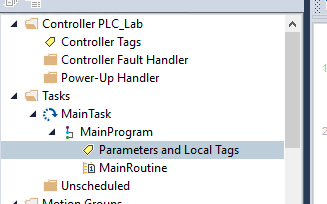
\includegraphics[width=3.2in]{BooleanTagCreation1}}
\caption{First step to creating a new boolean tag}
\label{fig:BooleanTagCreation1}
\end{figure}



\begin{figure}[h]
\centering
\textbf{Create new Boolean Tag}\par \medskip
\frame{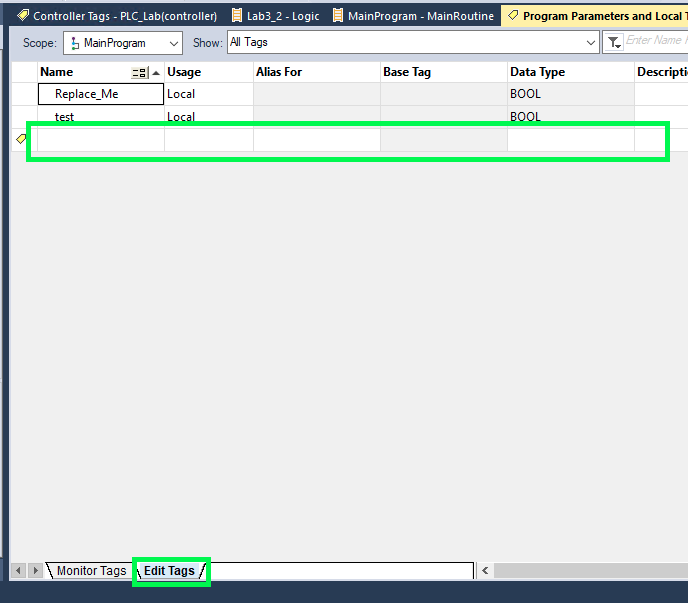
\includegraphics[width=3in]{EditTags}}
\caption{Second and Third step to creating a new boolean tag}
\label{fig:EditTags}
\end{figure}

\section{How to create a boolean tag}
\label{Section:BooleanTag}


To create another boolean tag to store the result of a boolean operation. Go to the left hand controller organizer menu. Under Main Program, double the item named Parameters and Local Tags. Refer to \figureautorefname \ref{fig:BooleanTagCreation1}.



Next, in the window that appears insure that you are on the edit tab of the parameters and tags window. In \figureautorefname \ref{fig:EditTags} you can see that the edit tab is in a green box for visibility at the bottom left. 

Finally, in the bottom entry in the list of tags enter the details for the tag that you are creating. The only two items that you should enter are the name and the datatype. The name must be a name that is not already taken and the datatype must be BOOL.

